\setcounter{equation}{0}
\section{Wave equation}
    Let us consider a pulse travelling on a string of linear mass density $\lambda$, with tension $T$.
    \begin{figure}[h!]
        \centering
        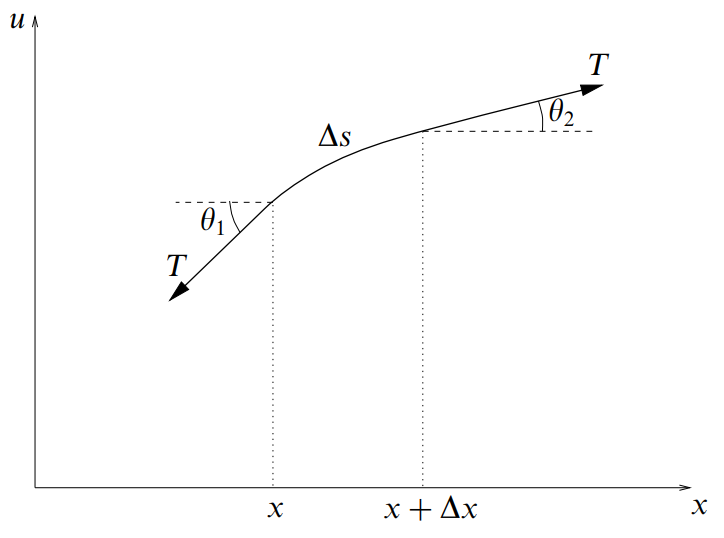
\includegraphics[width=0.5\textwidth]{figures/fig_string-pulse-segment.PNG}
    \end{figure}
    
    The figure above shows the forces acting on a segment of length $\Delta s$ on the string. The mass of the segment would be $\Delta m=\lambda\Delta s$. We find that the net upward force on this segment is
    \begin{align}
        \Delta F&=T\sin{\theta_2}-T\sin{\theta_1} \nonumber\\
        \implies\Delta F&=T\qty(\sin{\theta_2}-\sin{\theta_1}) \label{eqn:wave:seg-force}
    \end{align}
    Assuming that the angles $\theta_1$, $\theta_2$ are small, we have the approximations:
    \begin{align*}
        \sin{\theta_1}&\approx\tan{\theta_1}=\pdv{x}u(x,t) \\
        \sin{\theta_2}&\approx\tan{\theta_2}=\pdv{x}u(x+\Delta x,t)
    \end{align*}

    Now, given a function $f(x,t)$, its partial derivative is defined as
    \begin{align}
        \pdv{f}{x}=\dfrac{f(x+\Delta x,t)-f(x,t)}{\Delta x} \label{eqn:wave:pdv-defn}
    \end{align}
    If we consider $f(x,t)=\pdv{u}{x}$, then in equation (\ref{eqn:wave:pdv-defn}), we have
    \begin{align*}
        \pdv{x}\qty(\pdv{u}{x})&=\dfrac{\pdv{x}u(x+\Delta x,t)-\pdv{x}u(x,t)}{\Delta x} \\
        \implies\pdv{x}u(x+\Delta x,t)-\pdv{x}u(x,t)&=\pdv[2]{u}{x}\Delta x \\
        \implies\sin{\theta_2}-\sin{\theta_1}&=\pdv[2]{u}{x}\Delta x
    \end{align*}

    Inserting the above in equation (\ref{eqn:wave:seg-force}), we obtain
    \begin{align}
        \Delta F&=T\pdv[2]{u}{x}\Delta x \label{eqn:wave:seg-force-pdv}
    \end{align}

    The acceleration of the mass segment is given by $a=\pdv[2]{u}{t}$. Hence, by Newton's second law of motion, we have
    \begin{align}
        \Delta F&=\qty(\Delta m) a \nonumber\\
        \implies T\pdv[2]{u}{x}\Delta x&=\qty(\lambda\Delta s)\qty(\pdv[2]{u}{t})\qq{[using eqn. (\ref{eqn:wave:seg-force-pdv}) on LHS]} \label{eqn:wave:all-subs}
    \end{align}

    If the vibrations on the string are small, we can approximate:
    \begin{align*}
        \Delta s\approx\Delta x
    \end{align*}

    Therefore, in equation (\ref{eqn:wave:all-subs}), we have
    \begin{align}
        T\pdv[2]{u}{x}\Delta x&=\lambda\Delta x\pdv[2]{u}{t} \nonumber\\
        \implies\pdv[2]{u}{x}&=\dfrac{\lambda}{T}\pdv[2]{u}{t} \nonumber\\
        \implies\Aboxed{\pdv[2]{u}{x}&=\dfrac{1}{v^2}\pdv[2]{u}{t}} \label{eqn:wave-equation}
    \end{align}

    Equation (\ref{eqn:wave-equation}) is the \textit{wave equation}, where $v=\sqrt{\dfrac{T}{\lambda}}$ is the speed of the wave.